



% ============================================================
\section{Fine-tuning Large Discovery Models from Test-Time Search}
\label{sec:ldm-finetune}
% ============================================================

The framework above conducts discovery purely at inference time: sampling a large candidate pool, scoring it with the surrogate acquisition function $\acq_t$, and selecting candidates from the acquisition-tilted policy of Eq.~\eqref{eq:core}. While effective, this approach incurs the same substantial test-time computational overhead at every iterative round. The natural evolution is to \emph{amortise} this search directly into the model weights. In this paradigm, high-budget LDM test-time search (LDM-TTS) runs serve as an expert teacher, and fine-tuning distills a lightweight student model whose intrinsic policy already internalises the teacher's judgement on how to optimally allocate scarce experimental evaluations.




Crucially, as illustrated in Figure~\ref{fig:finetune-values}, modern LLM fine-tuning paradigms can be distinguished by the specific \emph{decision-theoretic value} they distill into the model's weights:
\begin{itemize}
    \item \textbf{Chat LLMs} distill \emph{human preference value} \citep{bai2022constitutional,rafailov2023direct}, aligning model behaviour with subjective human intuition, conversational helpfulness, and safety.
    \item \textbf{Reasoning LLMs} distill \emph{verification value} \citep{zelikman2022star}, training models to navigate closed-world, deterministic logical paths toward a verifiable ground-truth answer.
    \item \textbf{Discovery LLMs} distill \emph{epistemic acquisition value}. The goal is to cultivate a model-internal sense of \emph{research progress management} in open-ended, partially observed environments.
\end{itemize}

Consequently, the central object being distilled into our large discovery model is not the measured reward $R(x)$ alone, nor is it the static memorisation of a specific high-reward molecule, protein, or algorithmic solution. While recent works have successfully fine-tuned models against physical oracles—such as utilising docking scores for drug optimisation \citep{liu2025drugimprovergpt} or interatomic potentials for materials design \citep{cao2026reinforcement}—these approaches primarily train the model to exploit known reward landscapes. Our target is fundamentally different: we aim to \textbf{distill the underlying acquisition strategy itself}. As suggested by recent frameworks that integrate Gaussian Process likelihoods directly into LLM fine-tuning \citep{rankovic2025gollum}, teaching a model to recognise and act upon predictive uncertainty fundamentally restructures its latent representation of the domain.

In scientific discovery, the decision value of a move is inherently Bayesian: it balances predicted quality ($\mu_t$), epistemic uncertainty ($\sigma_t$), physical constraint satisfaction, and Pareto-frontier expansion. An experimental move can therefore be highly valuable even when it does not immediately maximise the posterior mean. This mirrors the counter-intuitive, high-information exploratory actions seen in breakthrough AI systems, such as AlphaZero's famous ``Move 37'' \citep{silver2017mastering,schut2025bridging}. A move is valuable because it resolves a critical unknown, opens a novel region of the search space, or alters the future trajectory of the research process. LDM fine-tuning aims to embed this hidden acquisition-value structure directly into the model's internal decision bias. By doing so, the model learns the strategic risk-taking required to manage an evolving research state, rather than merely imitating historical end solutions.







\begin{figure}[t]
\centering
\begingroup
\resizebox{0.98\textwidth}{!}{%
\begin{tikzpicture}[
    >={Latex[length=2.1mm]},
    font=\small,
    lane/.style n args={2}{draw=#1,line width=1.05pt,fill=#2,rounded corners=7pt,
        minimum width=43mm,minimum height=88mm}, % Increased height for better vertical spacing
    card/.style n args={2}{draw=#1,line width=0.9pt,fill=#2,rounded corners=5pt,
        align=center,inner sep=5pt,text width=35mm,minimum height=17mm}, % Increased height and width
    train/.style={draw=axisgray,line width=0.8pt,fill=white,rounded corners=4pt,
        align=center,inner sep=5pt,text width=35mm,minimum height=13mm}, % Increased height
    flow/.style={->,line width=0.9pt,draw=bodygray},
    title/.style={font=\bfseries\large,align=center},
    subtitle/.style={font=\scriptsize\itshape,align=center},
    note/.style={font=\scriptsize,align=center,text=bodygray},
]

\coordinate (C1) at (-5.15,0);
\coordinate (C2) at (0,0);
\coordinate (C3) at (5.15,0);

% Background lanes
\node[lane={chatredline}{chatred!30}] (lane1) at (C1) {};
\node[lane={reasonblueline}{reasonblue!32}] (lane2) at (C2) {};
\node[lane={discgreenline}{discgreen!40},line width=1.45pt] (lane3) at (C3) {};

% Titles
\node[title,text=chatdeep] at ($(C1)+(0,3.5)$) {Chat LLM};
\node[subtitle,text=chatredline] at ($(C1)+(0,3.0)$) {aligns with human priors};
\node[title,text=reasondeep] at ($(C2)+(0,3.5)$) {Reasoning LLM};
\node[subtitle,text=reasonblueline] at ($(C2)+(0,3.0)$) {navigates closed-world logic};
\node[title,text=discdeep] at ($(C3)+(0,3.5)$) {Discovery LLM};
\node[subtitle,text=discgreenline] at ($(C3)+(0,3.0)$) {explores open-world boundary}; % Updated text

% Value row
\node[card={chatredline}{white}] (human) at ($(C1)+(0,1.5)$)
  {\textbf{Preference value}\\subjective intuition,\\helpfulness, safety};
\node[card={reasonblueline}{white}] (logic) at ($(C2)+(0,1.5)$)
  {\textbf{Verification value}\\ground truth, tests,\\process verifiers};
\node[card={discgreenline}{white}] (acq) at ($(C3)+(0,1.5)$)
  {\textbf{Epistemic value}\\$\mu_t,\sigma_t$, information gain,\\Pareto expansion};

% Fine-tuning row
\node[train] (alignft) at ($(C1)+(0,-0.7)$)
  {\textbf{Alignment FT}\\distil human preferences};
\node[train] (reasonft) at ($(C2)+(0,-0.7)$)
  {\textbf{Reasoning FT}\\distil logical trajectories};
\node[train] (discft) at ($(C3)+(0,-0.7)$)
  {\textbf{Discovery FT}\\distil acquisition policy};

% Learned capability row
\node[card={chatredline}{chatred!12}] (assistant) at ($(C1)+(0,-2.8)$)
  {\textbf{Assistant}\\generate responses that\\satisfy user intent};
\node[card={reasonblueline}{reasonblue!14}] (solver) at ($(C2)+(0,-2.8)$)
  {\textbf{Solver}\\navigate paths to reach\\verifiable truth};
\node[card={discgreenline}{discgreen!18}] (manager) at ($(C3)+(0,-2.8)$)
  {\textbf{Research manager}\\propose experiments to\\maximise epistemic progress};

% Arrows
\foreach \a/\b in {human/alignft,alignft/assistant,logic/reasonft,reasonft/solver,acq/discft,discft/manager}{
  \draw[flow] (\a) -- (\b);
}

% Target annotation
\draw[discgreenline,line width=0.95pt,dashed,rounded corners=8pt]
  ($(lane3.south west)+(-0.10,-0.10)$) rectangle ($(lane3.north east)+(0.10,0.10)$);
\node[font=\small\itshape,text=discdeep,fill=white,inner sep=2pt]
  at ($(lane3.north)+(0,0.10)$) {our target};

\end{tikzpicture}%
}
\endgroup
\caption{\textbf{Fine-tuning as value distillation across model regimes.}
Chat LLMs distill human preference value to align with subjective intuition. Reasoning LLMs distill verification value to navigate deterministic proof paths. In contrast, Discovery LLMs distill epistemic acquisition value. Rather than merely memorising static, domain-specific solutions, discovery fine-tuning trains a research manager that learns an intrinsic acquisition strategy—prioritising high-information experiments to expand open-world boundaries and advance an evolving research trajectory.}
\label{fig:finetune-values}
\end{figure}







\subsection{Dataset Construction and Reasoning Augmentation}
\label{sec:dataset-construction}
% ============================================================

Figure~\ref{fig:training-pipeline} illustrates the end-to-end workflow of our training implementation, detailing how high-budget test-time search traces are processed, semantically augmented, and distilled into the fine-tuned Discovery LLM weights.

\begin{figure}[t]
\centering
\begingroup
\resizebox{0.98\textwidth}{!}{%
\begin{tikzpicture}[
    >={Latex[length=2.0mm]},
    font=\small,
    % Node styles
    stage/.style n args={2}{draw=#1, line width=1.1pt, fill=#2, rounded corners=8pt, inner sep=12pt},
    box/.style={draw=axisgray!80, line width=0.8pt, fill=white, rounded corners=5pt, align=center, inner sep=6pt, font=\small},
    accentbox/.style n args={2}{draw=#1, line width=0.9pt, fill=#2, rounded corners=5pt, align=center, inner sep=6pt, font=\small\bfseries},
    arrow/.style={->, line width=1.0pt, draw=bodygray},
    lbl/.style={font=\scriptsize\itshape, text=bodygray, align=center, fill=white, inner sep=3pt, rounded corners=2pt},
    title/.style={font=\bfseries\small, align=center}
]

% ============================================================
% STAGE 1: High-Budget Teacher Search
% ============================================================
\node[box] (history) at (0,0) {\textbf{Research Context} $\mathcal{C}_t$\\ \scriptsize (History, Observations)};

\node[box, right=0.6cm of history] (sampling) {\textbf{Candidate Pool Generation}\\ \scriptsize Sample $N$ candidates $\{\hat{x}_{t,i}\}_{i=1}^N \sim p_\theta(\cdot \mid \mathcal{C}_t)$};

\node[box, right=0.6cm of sampling] (surrogate) {\textbf{Surrogate BO Scoring}\\ \scriptsize Compute $\mu_t, \sigma_t, g_t \Rightarrow \alpha_t(\hat{x}_{t,i})$};

% Connectors Stage 1
\draw[arrow] (history) -- (sampling);
\draw[arrow] (sampling) -- (surrogate);

% Background Container 1
\begin{scope}[on background layer]
  \node[stage={reasonblueline}{reasonblue!15}, fit=(history) (sampling) (surrogate), label={[title, text=reasondeep]north:\textbf{Stage 1: High-Budget Test-Time Search (Teacher)}}] (stage1) {};
\end{scope}


% ============================================================
% STAGE 2: Dataset Construction & Reasoning Augmentation
% ============================================================
% Significantly expanded vertical gap to 3.8cm
\node[box, below=2.8cm of surrogate] (tilt) {\textbf{Empirical Policy Tilt}\\ \scriptsize Filter via $\widehat{\pi}_t^{(N)}(\hat{x}_{t,i}) \propto \exp\{\eta\,\alpha_t(\hat{x}_{t,i})\}$};

\node[accentbox={discgreenline}{discgreen!20}, left=0.6cm of tilt] (explain) {\textbf{Reasoning Augmentation}\\ \scriptsize $z_{t,i} = \operatorname{Explain}\left(\mathcal{C}_t, \hat{x}_{t,i}, \mu_t, \sigma_t, \alpha_t\right)$\\ \scriptsize \textit{(Translate BO stats to CoT rationale)}};

\node[box, left=0.6cm of explain] (dataset) {\textbf{SFT Dataset} $\mathcal{D}_{\text{SFT}}$\\ \scriptsize Tuples: $(\mathcal{C}_t, z_{t,i}, \hat{x}_{t,i})$};

% Connectors Stage 2
\draw[arrow] (surrogate) -- (tilt);
\draw[arrow] (tilt) -- (explain);
\draw[arrow] (explain) -- (dataset);

% Background Container 2
\begin{scope}[on background layer]
  \node[stage={discgreenline}{discgreen!18}, fit=(tilt) (explain) (dataset), label={[title, text=discdeep]north:\textbf{Stage 2: Dataset Construction \& Reasoning Augmentation}}] (stage2) {};
\end{scope}


% ============================================================
% STAGE 3: Policy Distillation & Deployment
% ============================================================
% Significantly expanded vertical gap to 3.8cm
\node[box, below=2.8cm of dataset] (basellm) {\textbf{Base LLM} $p_\theta$\\ \scriptsize (Un-tuned Reservoir)};

\node[box, right=0.6cm of basellm] (sftloss) {\textbf{Autoregressive SFT}\\ \scriptsize $\max_\theta \log p_\theta(z_{t,i} \mid \mathcal{C}_t) + \log p_\theta(\hat{x}_{t,i} \mid \mathcal{C}_t, z_{t,i})$};

\node[accentbox={chatredline}{chatred!25}, right=0.6cm of sftloss] (student) {\textbf{Discovery LLM} $p_{\text{SFT}}$\\ \scriptsize Amortised Research Manager\\ \scriptsize \textit{(Fast Low-Budget Inference)}};

% Connectors Stage 3
\draw[arrow] (dataset) -- (basellm);
\draw[arrow] (basellm) -- (sftloss);
\draw[arrow] (sftloss) -- (student);

% Background Container 3
\begin{scope}[on background layer]
  \node[stage={chatredline}{chatred!15}, fit=(basellm) (sftloss) (student), label={[title, text=chatdeep]north:\textbf{Stage 3: Supervised Fine-Tuning (Student Distillation)}}] (stage3) {};
\end{scope}

% Big Flow Arrows connecting stages
\draw[line width=1.5pt, ->, draw=discdeep, dashed] (stage1.south east) -- node[lbl] {Raw Search Traces} (stage2.north east);
\draw[line width=1.5pt, ->, draw=chatdeep, dashed] (stage2.south west) -- node[lbl] {Augmented Dataset} (stage3.north west);

\end{tikzpicture}%
}
\endgroup
\caption{\textbf{Overview of the LDM training pipeline workflow.}
\textbf{Stage 1:} High-budget test-time search generates candidate pools scored by surrogate acquisition values ($\alpha_t$). 
\textbf{Stage 2:} High-value candidates are filtered via an empirical policy tilt $\widehat{\pi}_t^{(N)}$, and numerical BO statistics are translated into semantic reasoning rationales ($z_{t,i}$) via reasoning augmentation. 
\textbf{Stage 3:} The base model is fine-tuned on the CoT target $(z_{t,i}, \hat{x}_{t,i})$ using standard next-token prediction, compiling the high-budget search policy into an amortised student model ($p_{\text{SFT}}$) capable of fast, low-budget inference.}
\label{fig:training-pipeline}
\end{figure}



Every round of Large Discovery Model Test-Time Search (LDM-TTS) produces significantly more training information than the single candidate eventually sent to the expensive physical oracle. The atomic training signal is not merely ``which candidate won,'' but a rich, local research decision: given the current context history, which possible next moves would advance the search, and why? 

At round $t$, the history $\C_t$ is used to generate a large candidate pool $\{\hat{x}_{t,i}\}_{i=1}^{N}$ from the base reservoir $p_{\theta}(\cdot\mid\C_t)$. The surrogate model then assigns each candidate predictive statistics and an acquisition score, yielding a rich tuple of features:
\[
  \left(
    \C_t,\ \hat{x}_{t,i},\ 
    \mu_t(\hat{x}_{t,i}),\ 
    \sigma_t(\hat{x}_{t,i}),\ 
    g_t(\hat{x}_{t,i}),\ 
    \acq_t(\hat{x}_{t,i})
  \right),
  \qquad i=1,\ldots,N,
\]
where $g_t$ denotes any additional value components relevant to the domain, such as constraint slack, evaluation cost, novelty, or hypervolume contribution. While only a small subset of these candidates receives a true expensive evaluation, \emph{all} candidates receive a cheap, surrogate-derived decision label. Thus, the surplus candidates created by test-time scaling are not wasted samples; they serve as counterfactual comparisons under identical histories. They reveal which research moves the LLM proposed, how the Bayesian optimisation (BO) value ranked them, and which trade-offs between exploitation, exploration, and frontier expansion were optimal at that specific stage of the search.

For a fixed candidate pool, the high-budget TTS teacher induces an empirical tilted distribution:
\begin{equation}
\label{eq:empirical-tilt}
  \widehat{\pi}^{(N)}_t(\hat{x}_{t,i})
  =
  \frac{\exp\{\eta\,\acq_t(\hat{x}_{t,i})\}}
       {\sum_{j=1}^{N}\exp\{\eta\,\acq_t(\hat{x}_{t,j})\}} .
\end{equation}
Increasing the pool size $N$ tightens the approximation to the ideal acquisition policy $\pi_t$. Consequently, low-budget search traces demonstrate the default biases of the base reservoir, while high-budget traces reveal the high-value regions reachable when that same reservoir is filtered aggressively by BO value. This is the discovery analogue of collecting reasoning traces from scaled test-time compute \citep{snellScalingLLMTestTime2024,wangTutorialLLMReasoning2025}, except the target value is supplied by a calibrated model of an expensive scientific objective rather than a cheap logical verifier.

\paragraph{Overcoming the Scalar Bottleneck.}
A practical difficulty in distilling Eq.~\eqref{eq:empirical-tilt} directly is that acquisition value is a compact numerical object. While the scalar $\acq_t(x)$ is precise for ranking, it obscures the \emph{semantic reason} why a candidate is useful for research progress. Asking a language model to internalise a complex policy purely from scalar weights creates an unnecessary bottleneck, as the model's strongest representation space is textual reasoning.

To bridge this modality gap, we introduce \emph{reasoning augmentation} as a core component of discovery dataset construction. Each test-time-search trace is augmented with a short acquisition rationale $z_{t,i}$ that verbalises why a candidate possesses high or low decision value:\label{sec:reasoning-augmentation}
\[
  z_{t,i}
  =
  \operatorname{Explain}
  \left(
    \C_t,\ \hat{x}_{t,i},\ 
    \mu_t(\hat{x}_{t,i}),\ 
    \sigma_t(\hat{x}_{t,i}),\ 
    g_t(\hat{x}_{t,i}),\ 
    \acq_t(\hat{x}_{t,i})
  \right).
\]
Crucially, this explanation is not an unconstrained, post-hoc hallucination. It is deterministically anchored to the surrogate's value decomposition. The rationale explicitly states whether the candidate exploits a high posterior mean, explores an under-modelled region (high variance), satisfies structural constraints, preserves batch diversity, or tests a novel hypothesis after a plateau in the reward landscape. 

Fine-tuning can then maximise the likelihood of both the rationale and the proposed action, for example:
\[
  \max_\phi
  \sum_t\sum_i
  \bar{w}_{t,i}
  \log p_\phi(z_{t,i},\hat{x}_{t,i}\mid\C_t),
\]
where $\bar{w}_{t,i}$ represents a normalised weight derived from $\widehat{\pi}^{(N)}_t$. Alternatively, $z_{t,i}$ can be utilised as an auxiliary target that is stripped during deployment. By using reasoning tokens to describe BO value in semantic terms, the model easily absorbs the underlying research-management rules rather than merely memorising isolated high-scoring designs. 

While this resembles chain-of-thought or process supervision, the supervised objective is fundamentally different. In standard reasoning fine-tuning, intermediate tokens explain \emph{how} to reach a correct answer in a closed problem. In discovery fine-tuning, intermediate tokens explain \emph{why} a proposed experiment is worth running under epistemic uncertainty. The rationale teaches the model how the strategic value of exploiting versus exploring depends dynamically on the current research state.

While this resembles chain-of-thought or process supervision, the supervised objective is fundamentally different. In standard reasoning fine-tuning, intermediate tokens explain \emph{how} to reach a correct answer in a closed problem. In discovery fine-tuning, intermediate tokens explain \emph{why} a proposed experiment is worth running under epistemic uncertainty. The rationale teaches the model how the strategic value of exploiting versus exploring depends dynamically on the current research state. 

Table~\ref{tab:reasoning-augmentation} provides concrete examples of how these numerical acquisition statistics are translated into semantic, trainable text across three distinct scientific domains.

\begin{table}[t]
\centering
\small
\begin{tabular}{@{}p{0.18\linewidth}p{0.36\linewidth}p{0.40\linewidth}@{}}
\toprule
\textbf{Domain} & \textbf{Acquisition evidence (Numerical)} & \textbf{Example augmented rationale (Semantic)} \\
\midrule
\texttt{autoresearch} code search &
Best run \texttt{state\_0019} reaches \texttt{val\_bpb} $0.9811$ by lowering \texttt{TOTAL\_BATCH\_SIZE} and tuning \texttt{ASPECT\_RATIO}; several near-best runs also lower the batch size. The current parent already sits at the minimum batch size with only $5$ active parameters and no improvement over the last $4$ rounds. &
Lowering the total batch size has been a robust positive move---more steps fit inside the fixed $30$\,s budget---but that lever is now exhausted and the active parameters have \textbf{plateaued over the last four rounds}, so the set is near its ceiling. Rather than re-tuning saturated knobs, I should \textbf{activate a currently-inactive parameter} (e.g.\ \texttt{MATRIX\_LR}) to open a new optimisation dimension. \\
\addlinespace
Antibody CDRH3 design &
Best sequence \texttt{ADGHTKQNPRW} at $-64.28$; the last four candidates share the fixed prefix \texttt{ADGHTKQNPR} and scan only the final position (W $-64.28$, Y $-62.69$, A $-59.38$, S $-57.96$). &
The history is a single-point scan of the last residue on an already-refined scaffold, with the bulky aromatic W best so far. The informative move is to keep the refined prefix and test an \textbf{untested residue of similar hydrophobic character}---leucine (L)---which may reproduce W's favourable hydrophobic contact; propose \texttt{ADGHTKQNPRL}. \\
\addlinespace
Small-molecule discovery &
$29$ molecules evaluated and the loop is flagged \texttt{stalled}; the top actives ($\sim\!8.1$) share one isoxazolone/thiazolone fused core with isopropoxy and cyano groups, docking $\sim\!-8$. &
Because the loop is stalled and near-duplicates are disallowed, adding a methyl to a known winner carries no information. The higher-value move is a \textbf{recombination or scaffold hop}---e.g.\ combining the pyridine-ring variant with the morpholine side chain into a molecule not yet seen---so the candidate probes a genuinely new region of the Pareto frontier rather than exploiting a saturated one. \\
\bottomrule
\end{tabular}
\vspace{0.5em}
\caption{\textbf{Reasoning augmentation turns numerical acquisition labels into semantic training signals.}
The rationales are faithful (translated, condensed) excerpts of actual reasoning traces generated by the
self-hosted DeepSeek V4 Flash teacher inside the high-budget LDM-TTS loop, one per domain. They describe the
epistemic value of managing research progress---reading the evaluated history, diagnosing stagnation, and
choosing an information-adding move---rather than focusing purely on the domain-specific final solution.}
\label{tab:reasoning-augmentation}
\end{table}


\subsection{Supervised Fine-Tuning for Policy Distillation}
\label{sec:sft-training}
% ============================================================

With the reasoning-augmented dataset constructed, the next step is to distil the high-budget test-time search policy into the weights of the base language model. We accomplish this through Supervised Fine-Tuning (SFT), effectively upgrading the generic base model into a domain-aware research manager.

Unlike standard alignment SFT, which performs behavioural cloning on human demonstrations, Discovery SFT trains the model to imitate the surrogate-guided, acquisition-tilted distribution. To construct the final SFT dataset $\mathcal{D}_{\text{SFT}}$, we filter or sample the candidate pools generated during test-time search. Rather than uniformly training on all generated candidates, we sample high-value trajectories $(\C_t, z_{t,i}, \hat{x}_{t,i})$ proportional to their empirical acquisition tilt $\widehat{\pi}^{(N)}_t(\hat{x}_{t,i})$ defined in Eq.~\eqref{eq:empirical-tilt}. Alternatively, one can apply a strict top-$k$ filter per round, retaining only the candidates that maximally expanded the Pareto frontier or possessed the highest epistemic value.

The base model parameters $\theta$ are then updated using standard autoregressive next-token prediction. Because we employ reasoning augmentation, the target sequence is structured as a Chain-of-Thought (CoT): the model must first generate the acquisition rationale $z_{t,i}$ before generating the actual experimental candidate $\hat{x}_{t,i}$. The SFT objective minimises the negative log-likelihood over the filtered trajectories:
\begin{equation}
\label{eq:sft-loss}
  \mathcal{L}_{\text{SFT}}(\theta)
  =
  -\mathbb{E}_{(\C_t, z_{t,i}, \hat{x}_{t,i}) \sim \mathcal{D}_{\text{SFT}}}
  \Big[ \log p_\theta(z_{t,i} \mid \C_t) + \log p_\theta(\hat{x}_{t,i} \mid \C_t, z_{t,i}) \Big].
\end{equation}

This factorisation is crucial for internalising the research-management policy. By enforcing that the rationale $z_{t,i}$ is predicted first, the subsequent generation of the candidate $\hat{x}_{t,i}$ becomes strongly conditioned on the semantic explanation of its epistemic value. The model learns to explicitly ``think'' about uncertainty, cost, and exploration before proposing an experimental structure. 

\paragraph{Amortising the Search Budget.}
During training, the base model is forced to map the observed research history $\C_t$ directly to high-acquisition actions. At inference time, the resulting fine-tuned model, $p_{\text{SFT}}$, generates high-quality proposals and accurate BO rationales natively, \emph{without} requiring the expensive test-time over-generation and surrogate scoring used by the teacher. 

In this way, SFT acts as a direct compilation of the test-time search loop into the network parameters. The model effectively internalises the BO acquisition landscape: it shifts its default sampling distribution from generic domain syntax toward the specific subspaces that maximise epistemic progress. While this SFT phase provides a robust initialisation, it also lays the necessary groundwork for further continuous refinement, such as direct preference optimisation against physical oracle feedback.






% ==========================================



\subsection{Expected effect on the LDM loop}
\label{sec:finetune-effect}

In the regret view of \S\ref{sec:theory-main}, fine-tuning acts on the two LLM-dependent terms. First, by
learning from successful search traces, the model can expand or shift its support $A_t$ toward regions that
high-budget LDM-TTS repeatedly found useful, reducing the discovery gap. Second, by assigning greater
probability to near-acquisition candidates, it increases the reservoir mass $\kappa_t(\zeta_t)$ in
Eq.~\eqref{eq:coverage}, reducing the sampling shortfall term. Operationally, the fine-tuned model should need
a smaller candidate pool $N$ to expose the same amount of acquisition-relevant mass.

This is why we view LDM fine-tuning as \emph{value distillation from discovery data}. The discovery data hides
a decision value that is only weakly and indirectly specified by ordinary language pretraining: how to read the
current research state, when to exploit a known promising region, when to explore an uncertain one, when to
maintain diversity, when to change the search support, and when to spend an expensive evaluation on an
informative rather than obviously best candidate. Fine-tuning does not remove the need for the surrogate,
because calibration must still be updated as new measurements arrive. Instead, it changes the LLM from a broad
semantic proposal prior into a research-progress prior: a model whose internal decision bias has absorbed part
of the acquisition value that was previously supplied only at test time. The experiments below ask whether this
amortised value improves discovery efficiency when the trained model is placed back inside the LDM loop.

\subsection{Fine-tuning experiments}
\label{sec:finetune-experiments}

\subsubsection{Cross-molecule transfer without reasoning augmentation}
\label{sec:finetune-no-augmentation}

We first test the minimal form of discovery fine-tuning, without the reasoning augmentation of
\S\ref{sec:reasoning-augmentation}. The training data are collected from a source molecular optimisation task
using high-budget LDM-TTS traces. We fine-tune the base Qwen3.5-9B proposer on the resulting discovery data
using acquisition-weighted examples, but do not include explicit semantic rationales $z_{t,i}$. The fine-tuned
model is then evaluated on a different molecular optimisation task and placed back inside the same
acquisition-guided LDM loop.

\textbf{Example training record without reasoning augmentation.}
The no-augmentation dataset still contains the full LDM state: target context, objective directions, design
constraints, evaluated history with oracle results, surrogate predictions and uncertainties, progress flags,
duplicate-avoidance constraints, and the requested action. The excerpt below keeps all feature types and omits
only additional history rows that repeat the same schema; for readability, the long raw \texttt{instruction}
string is rendered as parsed fields. The null \texttt{reasoning} field means no separate acquisition rationale
$z_{t,i}$ is prepended to the target.

\begin{lstlisting}[
basicstyle=\ttfamily\scriptsize,
breaklines=true,
columns=fullflexible,
keepspaces=true,
showstringspaces=false,
frame=single,
framerule=0.35pt,
aboveskip=3pt,
belowskip=4pt
]
{
  "system": "You are a scientific search agent proposing candidate molecules under an iterative multi-objective Bayesian optimization loop. Return ONLY the JSON action. Never predict docking score, activity, EHVI, uncertainty, or rank.",
  "instruction": {
    "task": "smallmol (molecule)",
    "target": "KRAS G12D small-molecule candidates",
    "target_context": "switch-II pocket context; do not copy known drugs or exact chemotypes",
    "objectives": [
      {"name": "vina_docking", "direction": "minimize", "source": "AutoDock Vina docking score"},
      {"name": "neural_activity", "direction": "maximize", "source": "target-specific activity model"}
    ],
    "design_space": {
      "representation": "complete_design", "active_parameters": [], "new_parameters_may_be_invented": true,
      "constraints": {"format": "single-component organic SMILES", "smiles_max_len": 80,
        "avoid": ["salts", "dot-disconnected mixtures", "reaction arrows", "atom maps", "metals", "isotopes", "radicals", "charged salts"]}
    },
    "observed_history": [
      {"design": "CC(C)Oc1ccc(C#N)c2oc(=O)n(CCC#N)c12", "roles": ["evaluated"],
       "results": {"vina": -8.313, "activity": 7.9656199377728925},
       "surrogate": {"predicted_mean": [-7.895168304443359, 7.713257312774658],
                     "uncertainty": [0.35512545704841614, 0.5342587232589722]}}
      // 28 further "evaluated" entries with the same {results, surrogate} schema, omitted here
    ],
    "evaluations_so_far": 29,
    "progress": {"stalled": true, "rounds_since_improvement": null,
      "description": "Avoid simple extensions or near-copies of recent_selected; use other Pareto/extreme/balanced parents and vary the edit type."},
    "do_not_repeat": ["O=c1[nH]c2ccccc2s1", "N#Cc1cccc2sc(=O)[nH]c12"],  // all 29 previously evaluated SMILES
    "move": {"allowed_actions": ["propose"], "number_of_candidates": 7, "candidate_limit": 8,
      "operator": "elite crossover and scaffold hop", "diversity_alert": "avoid simple extensions or near-copies of recent_selected"}
  },
  "input": "",
  "output": {
    "type": "propose",
    "reasoning": null,
    "payload": {"candidates": [
      {"design": "CC(C)Oc1ncc(C#N)c2oc(=O)n(CCCN3CCOCC3)c12", "rationale": "recombine pyridine and morpholine"},
      {"design": "CN1C(=O)oc2c(C#N)cnc(C3CC3CO)c21", "rationale": "methyl substituent with cyclopropylmethanol"}
      // 5 further candidates with the same {design, rationale} schema, omitted here
    ]},
    "summary": null
  },
  "source": "smallmol"
}
\end{lstlisting}

This setting shows positive transfer across molecular tasks. The base
Qwen3.5-9B LDM reaches a final hypervolume of $16.489\pm5.867$, while the fine-tuned model reaches
$22.279\pm3.828$ under the same evaluation protocol. The improvement is substantial: fine-tuning on
acquisition-tilted discovery data lifts the base proposer by nearly six hypervolume units and closes most of
the gap to the much larger DeepSeek V4 Flash reference ($24.548\pm3.589$), while also sharply reducing the
seed-to-seed variance. Because the discovery data are collected from one molecule and tested on another, the
gain cannot be explained simply as memorising the final molecules in the training task. Instead, it supports the
central value-distillation picture: even without explicit reasoning augmentation, fine-tuning can transfer part
of the acquisition-biased research-management policy into the model weights.

\subsubsection{Fine-tuning with reasoning-augmented discovery data}
\label{sec:finetune-with-augmentation}
The second setting augments the same discovery records with an explicit research-progress trace before the
final JSON action. Crucially, both the underlying search traces and the reasoning augmentation are produced by
the \emph{same} model family: the high-budget LDM-TTS rollouts that generate the candidate pools and their
acquisition-tilted labels are collected using a self-hosted \emph{DeepSeek V4 Flash} proposer inside our LDM
framework, and the same self-hosted DeepSeek V4 Flash teacher is then used to translate the numerical and
structural state of the LDM loop into natural-language reasoning: what has been learned from the evaluated
history, why the current search is stalled, which fragments or scaffold families appear useful, and which next
edits represent genuine research moves rather than near-duplicates. Using a single self-hosted teacher for both
rollout and rationale generation keeps the reasoning trace $z_t$ faithfully aligned with the acquisition
decisions actually taken during search, rather than importing an external model's post-hoc narration.

\begin{tcolorbox}[
    enhanced,
    breakable,
    colframe=discgreenline,
    colback=discgreen!18,
    boxrule=0.9pt,
    arc=4pt,
    left=8pt,
    right=8pt,
    top=7pt,
    bottom=7pt
]
{\large\bfseries Reasoning augmentation makes the research-progress trace part of the training target.}
\[
  {\Large 
\texttt{<think>}~z_t~\texttt{</think>}
  \quad\Vert\quad
  \texttt{\{JSON action\}}}
\]
\small
Here $z_t$ is not an optional explanation shown only for interpretability. It is supervised text generated by a
strong teacher, and it trains the student to recognise stalled search, identify transferable molecular motifs,
choose non-duplicate edit types, and manage the exploration--exploitation trade-off before emitting candidates.
\end{tcolorbox}

Thus, the student is trained not only to emit candidate molecules, but also to internalise the policy for
managing an evolving discovery trajectory. Unlike the no-augmentation record in
\S\ref{sec:finetune-no-augmentation}, the reasoning text is part of the supervised target. The short
per-candidate \texttt{rationale} fields remain ordinary action-schema metadata; the added supervision is the
full trace $z_t$ that explains the research progress in semantic terms.

\textbf{What reasoning augmentation changes.}
Reasoning augmentation is a strictly \emph{additive} edit to the record of
\S\ref{sec:finetune-no-augmentation}: the \texttt{system} prompt, the \texttt{instruction} (the same 29-molecule
KRAS G12D state with oracle results, surrogate means and uncertainties, duplicate constraints and stalled-progress
flag), the proposed \texttt{payload.candidates}, and the action \texttt{type} are \emph{byte-for-byte identical}.
The only difference is that the \texttt{reasoning} field, which was \texttt{null} in the no-augmentation record,
is now populated with the research-progress trace $z_t$ that the model must generate \emph{before} the candidates.
Presenting the two records side by side therefore isolates the augmentation exactly: everything the model
conditions on and everything it must emit as an action is held fixed, and the supervised target gains only the
reasoning that precedes the action.

\begin{lstlisting}[
basicstyle=\ttfamily\scriptsize,
breaklines=true,
columns=fullflexible,
keepspaces=true,
showstringspaces=false,
frame=single,
framerule=0.35pt,
escapeinside={(*@}{@*)},
aboveskip=3pt,
belowskip=4pt
]
"output": {
  "type": "propose",
  (*@\color{gray}// no-augmentation record (\S\ref{sec:finetune-no-augmentation}): "reasoning": null@*)
  (*@\color{blue}\bfseries "reasoning": [        // reasoning augmentation fills exactly this field@*)
  (*@\color{blue}\bfseries    "Identify the research state: KRAS G12D small-molecule optimization with two objectives, lower Vina docking score and higher neural activity.",@*)
  (*@\color{blue}\bfseries    "Use the 29 evaluated molecules to infer that the search is stalled; avoid simple repetition or local extension of recent selections.",@*)
  (*@\color{blue}\bfseries    "Recognize a useful family: fused oxazolone/thiazolone-like cores with isopropoxy, cyano substitution, and N-substituents such as cyanopropyl or methyl.",@*)
  (*@\color{blue}\bfseries    "Do not copy the current elites directly. Instead, use recombination and scaffold hopping to produce proposal-reservoir moves.",@*)
  (*@\color{blue}\bfseries    "Combine evidence across parents: pyridine-ring analogues, morpholine side chains, cyclopropylmethanol motifs, halogen variants, and thiazolone/oxazolone core swaps.",@*)
  (*@\color{blue}\bfseries    "Return candidates as hypotheses for the external BO selector, not as score predictions or labels."@*)
  (*@\color{blue}\bfseries ],@*)
  "payload": { "candidates": [ (*@\color{gray}/* the same 7 SMILES candidates as the no-augmentation record */@*) ] },
  "summary": null
}
\end{lstlisting}

\paragraph{Comparison analysis: what the added supervision buys.}
Because the two records differ only in this one field, the comparison pinpoints what fine-tuning actually
learns from reasoning augmentation. In the no-augmentation record the model is trained to map the research
context $\C_t$ directly to the candidate list, with the intermediate acquisition judgement left implicit; the
loss $-\log p_\theta(\hat{x}_{t,i}\mid\C_t)$ never sees \emph{why} those candidates are good research moves. In
the augmented record the target factorises as
$-\big[\log p_\theta(z_{t,i}\mid\C_t) + \log p_\theta(\hat{x}_{t,i}\mid\C_t, z_{t,i})\big]$: the model must first
verbalise a faithful state assessment---the search has stalled, which scaffold family is transferable, that
elites must not be copied, that recombination/scaffold-hopping is the right operator---and then emit candidates
\emph{conditioned on} that assessment. The candidates themselves are unchanged, so the augmentation does not
teach new chemistry; it teaches the model \emph{when} and \emph{why} to make each kind of move. This is exactly
the capability that the small-molecule ablation (Table~\ref{tab:smallmol-cot}) shows is dormant in an un-tuned
backbone and only becomes valuable once it has been supervised into the weights, and that the deployment-time
trace in \S\ref{sec:finetune-cot-ablation} shows the fine-tuned model executing online.

\begin{figure}
    \centering
    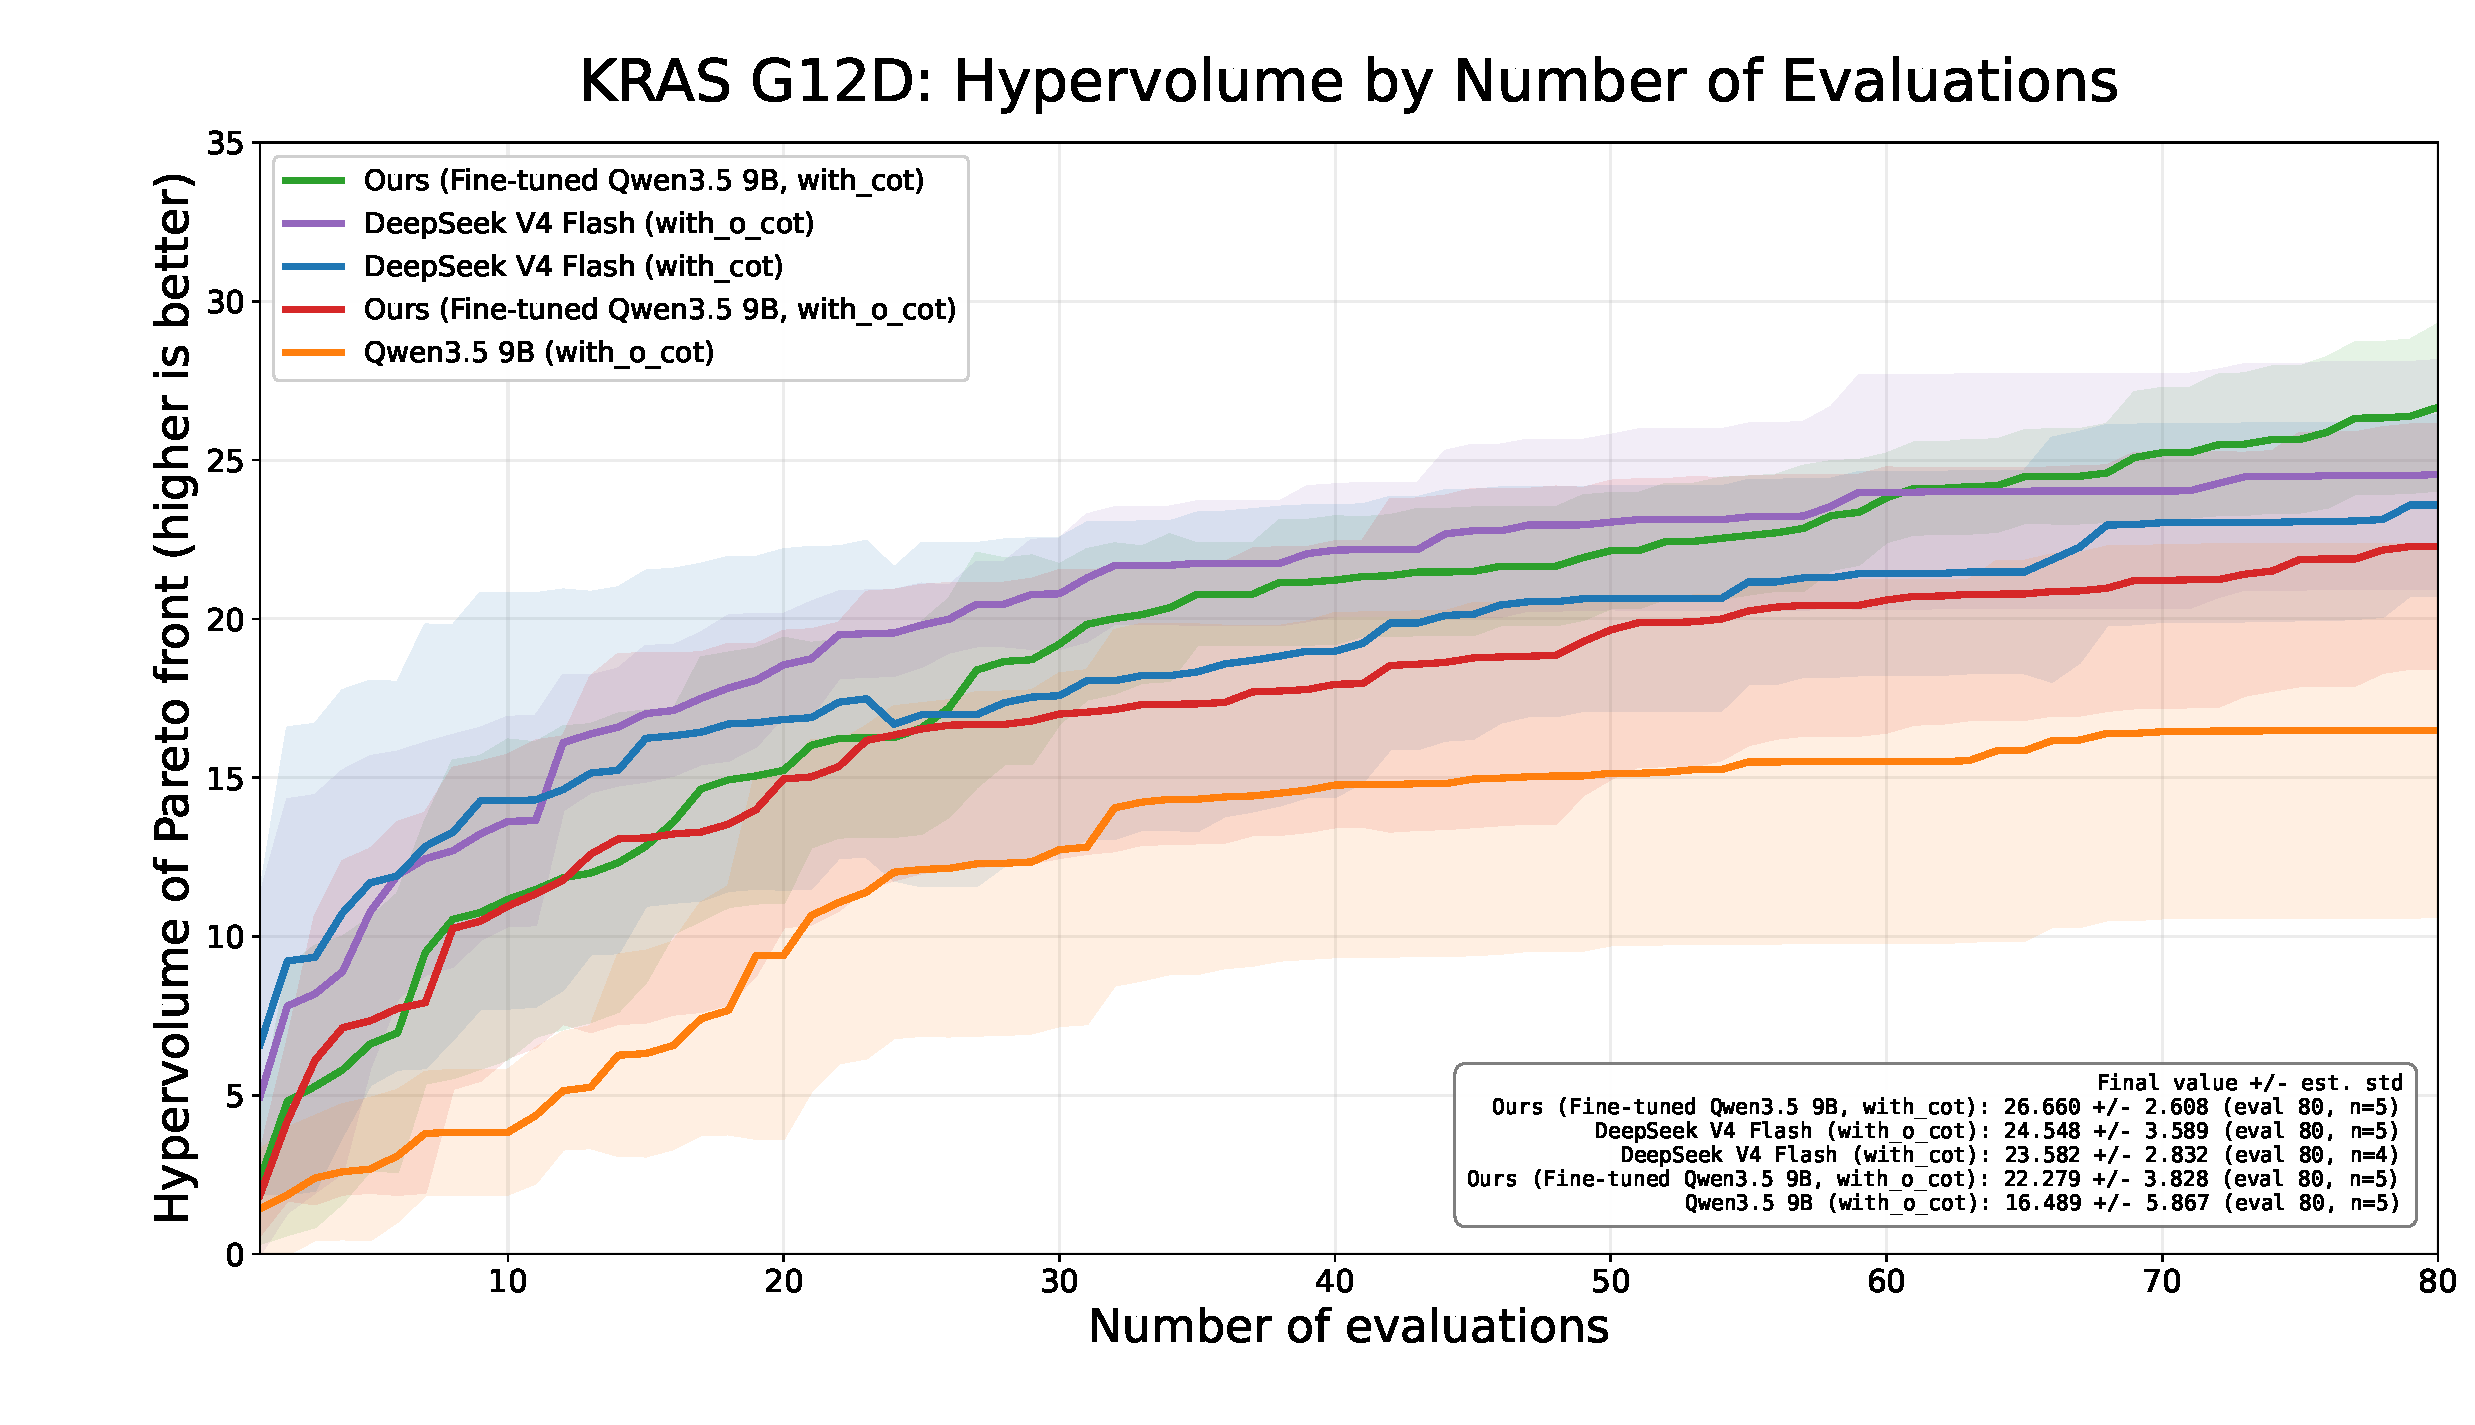
\includegraphics[width=0.92\linewidth]{figure/ldm_sft_small.pdf}
    \caption{\textbf{Fine-tuning with reasoning-augmented discovery data (KRAS G12D).} Best-so-far Pareto-front
    hypervolume against the number of expensive evaluations, averaged over five seeds ($\eta=6\mathrm{k}$
    proposer pool, BO batch 32, reference point $(0,5)$); shaded bands denote one standard deviation. Five
    inference-time policies are compared inside the identical acquisition-guided LDM loop: our reasoning-augmented
    fine-tuned Qwen3.5-9B (\emph{with\_cot}), the same student without the reasoning channel (\emph{without\_cot}),
    the self-hosted DeepSeek V4 Flash teacher with and without reasoning, and the un-tuned Qwen3.5-9B base
    proposer. The reasoning-augmented student attains the highest final hypervolume ($26.66\pm2.61$),
    \emph{surpassing the much larger DeepSeek V4 Flash teacher} that generated its training traces
    ($24.55\pm3.59$ without and $24.07\pm3.12$ with reasoning), while the un-tuned base proposer trails far
    behind ($16.49\pm5.87$).}
    \label{fig:finetune-cot-transfer}
\end{figure}

Figure~\ref{fig:finetune-cot-transfer} reports the small-molecule instance of the reasoning-augmentation
ablation on KRAS G12D, and Table~\ref{tab:smallmol-cot} lists final hypervolumes for both the G12C and G12D
targets. Four observations stand out. \textbf{(1) Fine-tuning transfers the acquisition policy:} the un-tuned
Qwen3.5-9B base proposer reaches only $16.49$ (G12D) / $11.64$ (G12C), while discovery fine-tuning lifts the
same backbone to $22.28$ / $14.73$ even \emph{without} a reasoning trace, confirming that acquisition-tilted
data alone compiles part of the search policy into the weights. \textbf{(2) The reasoning channel is the
dominant factor:} adding the \texttt{<think>}\,$z_t$\,\texttt{</think>} target lifts the fine-tuned student from
$22.28\!\to\!26.66$ on G12D ($+4.4$) and $14.73\!\to\!20.98$ on G12C ($+6.3$)---a larger jump than fine-tuning
without reasoning provides. \textbf{(3) The student surpasses its own teacher:} the reasoning-augmented 9B
student ($26.66$ / $20.98$) exceeds the self-hosted DeepSeek V4 Flash teacher that produced its training
rollouts ($24.55$ / $18.97$), despite the teacher being far larger. This is the amortisation claim realised:
distilling high-budget acquisition-tilted search into weights yields a compact model whose low-budget inference
policy is stronger than the expensive teacher loop it was distilled from. \textbf{(4) Reasoning value is
unlocked by fine-tuning, not intrinsic to the backbone:} for the un-tuned DeepSeek teacher, enabling the
reasoning channel is roughly neutral (G12D $24.55\!\to\!24.07$; G12C $18.97\!\to\!19.98$), whereas the same
channel yields a large gain once the model has been fine-tuned on reasoning-augmented discovery data. The
augmented trace does not merely help \emph{any} model narrate its choices; it teaches the student a specific
research-management policy that its native reasoning does not already contain.

\begin{table}[t]
\centering
\small
\begin{tabular}{@{}lcc@{}}
\toprule
\textbf{Inference policy (small-molecule LDM loop)} & \textbf{KRAS G12C} & \textbf{KRAS G12D} \\
 & HV $\uparrow$ & HV $\uparrow$ \\
\midrule
Qwen3.5-9B base (without\_cot)                 & $11.64\pm2.63$ & $16.49\pm5.87$ \\
Ours: fine-tuned Qwen3.5-9B (without\_cot)     & $14.73\pm3.09$ & $22.28\pm3.83$ \\
DeepSeek V4 Flash teacher (without\_cot)       & $18.97\pm1.76$ & $24.55\pm3.59$ \\
DeepSeek V4 Flash teacher (with\_cot)          & $19.98\pm2.00$ & $24.07\pm3.12$ \\
\textbf{Ours: fine-tuned Qwen3.5-9B (with\_cot)} & $\mathbf{20.98\pm2.92}$ & $\mathbf{26.66\pm2.61}$ \\
\bottomrule
\end{tabular}
\vspace{0.4em}
\caption{\textbf{Reasoning-augmentation ablation on small-molecule discovery.} Final Pareto-front hypervolume
(higher is better) at an evaluation budget of 80, averaged over five seeds, for both KRAS targets. The
reasoning-augmented fine-tuned student is best on both targets and surpasses the larger DeepSeek V4 Flash
teacher that generated its training data.}
\label{tab:smallmol-cot}
\end{table}

\paragraph{Why does chain-of-thought help discovery?}
The ablation isolates a specific answer to this question, and it is not the generic ``more test-time tokens
help'' effect reported for closed-ended reasoning benchmarks. Table~\ref{tab:smallmol-cot} shows that the
reasoning channel is \emph{worth almost nothing on its own}: enabling chain-of-thought on the un-tuned models
leaves performance essentially flat (the DeepSeek teacher moves $24.55\!\to\!24.07$ on G12D and
$18.97\!\to\!19.98$ on G12C, i.e.\ within noise). The same reasoning channel becomes strongly beneficial only
\emph{after} discovery fine-tuning, where it lifts our student by $+4.4$ (G12D) and $+6.3$ (G12C) hypervolume.
The gain from reasoning is therefore not a property of the tokens themselves but of \emph{what the model has
learned to compute in them}.

We attribute this to the difference between the two supervised objectives discussed in
\S\ref{sec:reasoning-augmentation}. In closed-ended reasoning, chain-of-thought helps because intermediate
tokens carry out a \emph{verifiable computation} toward a ground-truth answer, so a base model already
pretrained on such traces benefits immediately. In discovery, the useful intermediate computation is a
\emph{Bayesian acquisition judgement}---reading the evaluated history, estimating whether the search has
stalled, weighing predicted quality $\mu_t$ against epistemic uncertainty $\sigma_t$ and Pareto-front
expansion, and deciding whether the next move should exploit, explore, or restructure the search. This
computation is only weakly and indirectly specified by ordinary language pretraining, so an un-tuned model's
chain-of-thought verbalises plausible-sounding but acquisition-agnostic chemistry and does not change which
candidate it ultimately proposes. Discovery fine-tuning on reasoning-augmented traces
(Eq.~\eqref{eq:sft-loss}) supervises exactly this hidden computation: because the target factorises as
$\log p_\theta(z_{t,i}\mid\C_t) + \log p_\theta(\hat{x}_{t,i}\mid\C_t,z_{t,i})$, the candidate is generated
\emph{conditioned on} an acquisition rationale, and minimising the loss forces the model to first produce a
faithful research-state assessment and then act on it. The essential effect is a change of \emph{modality}:
the acquisition verdict---the surrogate's $(\mu_t,\sigma_t,\alpha_t)$ arithmetic that decides exploit
vs.\ explore vs.\ restructure---is an \emph{implicit, numerical} computation that an un-tuned model can at best
carry latently and inconsistently. Reasoning augmentation re-expresses it as an \emph{explicit, textual}
computation performed in the model's strongest representation space: the model now writes out, in words, the
direction the acquisition function points---which history evidence matters, whether the search has stalled, and
why the chosen move trades exploitation for exploration or frontier expansion. Fine-tuning is what installs this
translation from latent numerics to legible acquisition-direction analysis. After fine-tuning, the
chain-of-thought is no longer decorative narration; it is the surface on which the otherwise-hidden acquisition
computation is actually carried out---the inference-time execution of the distilled acquisition policy, which is
why it recovers a large fraction of the value that the high-budget teacher search supplied only through explicit
surrogate scoring. In short, chain-of-thought helps discovery not by adding generic deliberation, but by giving
the fine-tuned model a channel in which to \emph{run} the Bayesian research-management policy it was trained to
internalise.

\paragraph{Argument 1 (mechanism): CoT supplies the otherwise-hidden Bayesian acquisition computation.}
For closed-ended reasoning (math, code), the intermediate tokens carry a \emph{verifiable} computation toward a
ground-truth answer, which base pretraining already supplies---so an un-tuned model benefits immediately. For
\emph{discovery}, the useful intermediate computation is instead a \emph{Bayesian acquisition judgement}: read
the evaluated history, decide whether the search has stalled, weigh predicted quality against uncertainty and
Pareto-front expansion, and choose exploit vs.\ explore vs.\ restructure. Pretraining barely teaches this. The
factorised SFT objective $\log p_\theta(z_{t,i}\mid\C_t)+\log p_\theta(\hat{x}_{t,i}\mid\C_t,z_{t,i})$ forces the
model to \emph{first assess the research state and then act on it}, converting the surrogate's
\emph{implicit, numerical} $(\mu_t,\sigma_t,\alpha_t)$ arithmetic into an \emph{explicit, textual} acquisition
computation performed in the model's strongest representation space.

\subsubsection{In-distribution single-task fit}
\label{sec:finetune-indist}

Before evaluating the distilled policies inside the acquisition loop, we verify that supervised fine-tuning
actually absorbs each domain's reasoning-augmented data. We fine-tune one single-task model per domain and track
the training loss together with the held-out (in-distribution) evaluation loss; Figure~\ref{fig:indist-curves}
shows all three domains---\texttt{autoresearch} program search, small-molecule KRAS design, and antibody CDRH3
design. All fit cleanly: the loss collapses within the first few dozen steps and the held-out curve tracks the
training curve closely, indicating that the model absorbs the acquisition-annotated targets without over-fitting.
The absolute held-out loss differs by domain---$0.06$ for \texttt{autoresearch}, whose action space is a small
set of structured program edits, $0.38$ for small-molecule SMILES design, and $0.70$ for antibody CDRH3, whose
targets are free residue strings paired with longer acquisition rationales---but in every case the small
train--eval gap confirms that the in-distribution policy is learned faithfully. This establishes that any performance difference
later observed inside the loop reflects how the policy is \emph{used}, not a failure to fit the data.

\begin{figure}[t]
\centering
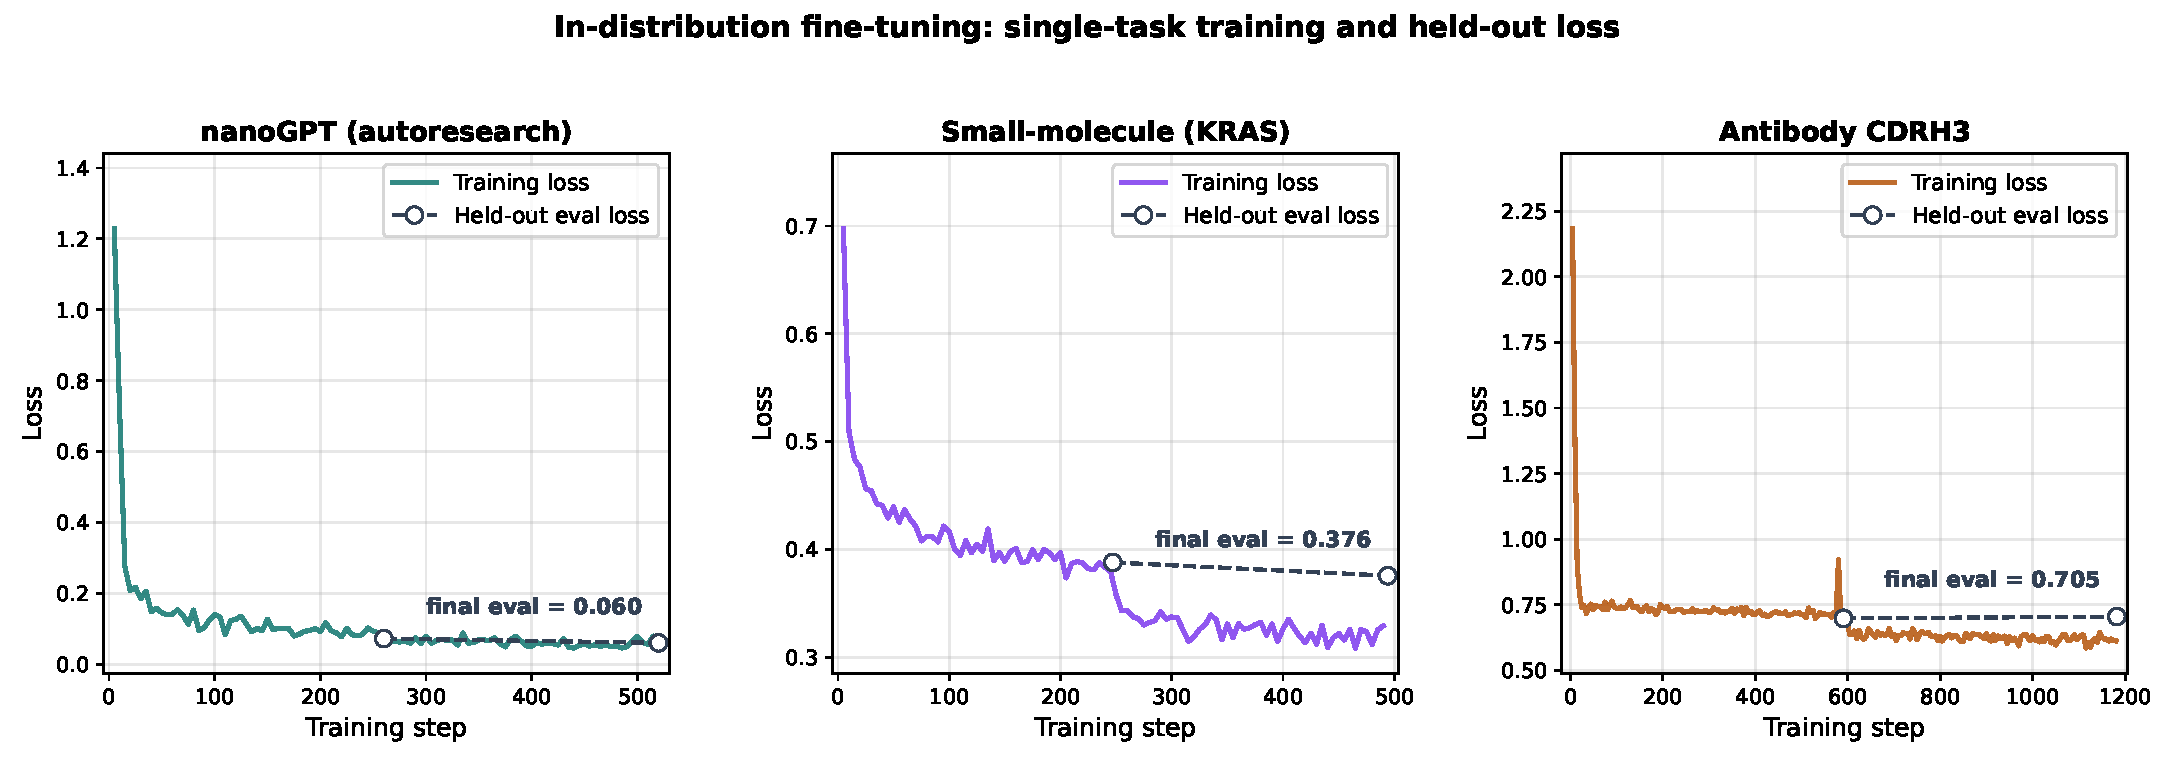
\includegraphics[width=0.95\linewidth]{figure/indist_curves.pdf}
\caption{\textbf{In-distribution single-task fine-tuning.} Training loss (solid) and held-out evaluation loss
(markers) versus training step for the \texttt{autoresearch}, small-molecule, and antibody CDRH3 policies. All
three converge within a few dozen steps and the held-out loss tracks the training loss, confirming a faithful
in-distribution fit before the acquisition-loop evaluations.}
\label{fig:indist-curves}
\end{figure}

\subsubsection{Cross-domain reasoning-augmentation ablation and analysis}
\label{sec:finetune-cot-ablation}

The small-molecule study above establishes that reasoning augmentation is compatible with discovery
fine-tuning, but it leaves open the central question: \emph{does the reasoning trace itself contribute to
discovery performance, or is the gain attributable solely to weight-level exposure to acquisition-tilted
data?} To isolate the effect of the reasoning channel, we run a controlled $2\times2$ ablation across all
three domains---\texttt{autoresearch} program search, antibody CDRH3 design, and small-molecule
optimisation---crossing \textbf{base vs.\ fine-tuned} weights with \textbf{reasoning on vs.\ off} at inference
time. Concretely, the four conditions are: (i) the un-tuned Qwen3.5-9B proposer with chain-of-thought enabled;
(ii) the same base model with thinking suppressed; (iii) the discovery-fine-tuned model emitting the
\texttt{<think>}\,$z_t$\,\texttt{</think>}\,$\Vert$\,\texttt{JSON} target of \S\ref{sec:finetune-with-augmentation};
and (iv) the fine-tuned model with the thinking block suppressed so that it emits the JSON action directly.
Because all four conditions are evaluated inside the identical acquisition-guided LDM loop with the same oracle
budget, any performance difference is attributable to the reasoning channel and the distilled policy rather
than to the search harness.

An important methodological point is that our teacher signal is generated \emph{end-to-end} by a single
self-hosted model. The high-budget LDM-TTS rollouts that produce the candidate pools and their
acquisition-tilted labels are collected with a self-hosted DeepSeek V4 Flash proposer operating inside our own
LDM framework, and the reasoning augmentation $z_t$ is generated by the same self-hosted DeepSeek V4 Flash
model conditioned on the surrogate's value decomposition. Keeping rollout and rationale under one self-hosted
teacher ensures the supervised reasoning is faithful to the acquisition decisions actually taken during search,
and avoids the confound of narrating one model's trajectory with a different, externally hosted model.

\paragraph{Qualitative evidence: the reasoning trace performs research-progress management.}
Because the deployment-time reasoning tokens are recorded, we can inspect what the fine-tuned model actually
``thinks'' before it acts. The trace below is a verbatim (translated) deployment-time rationale emitted by the
fine-tuned model on the \texttt{autoresearch} task, immediately before it issued an
\texttt{expand\_design\_space} action. It is not a training example; it is generated online inside the LDM loop.

\begin{tcolorbox}[
    enhanced,
    breakable,
    colframe=discgreenline,
    colback=discgreen!18,
    boxrule=0.9pt,
    arc=4pt,
    left=8pt,
    right=8pt,
    top=7pt,
    bottom=7pt
]
{\bfseries Deployment-time reasoning trace (\texttt{autoresearch}, fine-tuned student).}\\[2pt]
\small
{\bfseries Model reasoning} $z_t$: ``The best result so far is \texttt{state\_0019} (\texttt{val\_bpb}=0.98811),
which lowered \texttt{TOTAL\_BATCH\_SIZE} from 524288 to 262144; edits to \texttt{ASPECT\_RATIO},
\texttt{EMBEDDING\_LR}, and \texttt{HEAD\_DIM} did not beat it, so the current active parameter space is likely
near a local optimum and further tuning of these knobs has limited upside. However, the matrix parameters---the
attention and MLP weights that make up most of the model and are optimised by Muon via \texttt{MATRIX\_LR}---sit
in the inactive list, so the surrogate has never been allowed to model their effect. Activating \texttt{MATRIX\_LR}
would immediately expand the surrogate's feature space and let subsequent candidates jointly tune the embedding,
matrix, and unembedding learning rates. I will activate it at its current value 0.04, so no abrupt change is
introduced while the option to optimise it is opened up.''

\smallskip
{\bfseries Emitted action}:\\
{\ttfamily\scriptsize \{"type": "expand\_design\_space",}\\
{\ttfamily\scriptsize \ "payload": \{"activate": "MATRIX\_LR", "initial\_value": 0.04\}\}}
\end{tcolorbox}

This trace exhibits precisely the epistemic-acquisition behaviour that \S\ref{sec:ldm-finetune} argues discovery
fine-tuning should distil. The model (i) reads the current research state from the evaluated history, (ii)
diagnoses a \emph{plateau} in the active design space, (iii) identifies a high-information but under-modelled
lever (a parameter the surrogate cannot yet see), and (iv) chooses a design-space \emph{expansion} rather than a
myopic exploitation edit---seeding the new coordinate conservatively to preserve the current best. This is
research-progress management, not memorisation of a high-reward configuration: the valuable move is the one that
resolves a structural unknown and reshapes the next phase of search.

\paragraph{Argument 2 (deployment): the model actually runs research-progress management online.}
The verbatim deployment-time trace above is generated \emph{inside the loop}, not retrieved from training. The
fine-tuned student (i) reads the current research state from the evaluated history, (ii) diagnoses a
\emph{plateau} in the active design space, (iii) identifies a high-information but under-modelled lever the
surrogate cannot yet see (\texttt{MATRIX\_LR}), and (iv) chooses a design-space \emph{expansion} over a myopic
exploitation edit. This is an acquisition-driven explore/restructure decision---the distilled policy executing
at inference time---not recall of a memorised high-reward configuration.

\paragraph{Quantitative comparison.}
Figure~\ref{fig:nanogpt-finetune-cot} shows the \texttt{autoresearch} instance of the ablation, and
Table~\ref{tab:finetune-cot-ablation} summarises the $2\times2$ result. Two consistent trends emerge. First,
discovery fine-tuning improves over the base proposer: with reasoning held on, fine-tuning lowers the best
validation bits-per-byte from $0.9825$ (base) to $0.9788$. Second, the reasoning channel is the decisive
factor and its value is again unlocked by fine-tuning: it lifts the base model only marginally
($0.9965\!\to\!0.9825$ once search is allowed to proceed) but is what lets the fine-tuned model reach the best
result overall. The reasoning-augmented fine-tuned student ($0.9788$) even edges below the much larger
Qwen3-Coder-30B reference proposer supplied with the full hyperparameter schema ($0.9801$), mirroring the
student-surpasses-teacher effect seen in the small-molecule study. Inspection of the traces shows why: only the
reasoning-enabled configurations reliably diagnose a plateau and act on it (e.g.\ the design-space expansion in
the box above), whereas thinking-suppressed runs stall early---the \texttt{no CoT} base curve flattens near
$0.9965$ within ten iterations.

\begin{figure}[t]
\centering
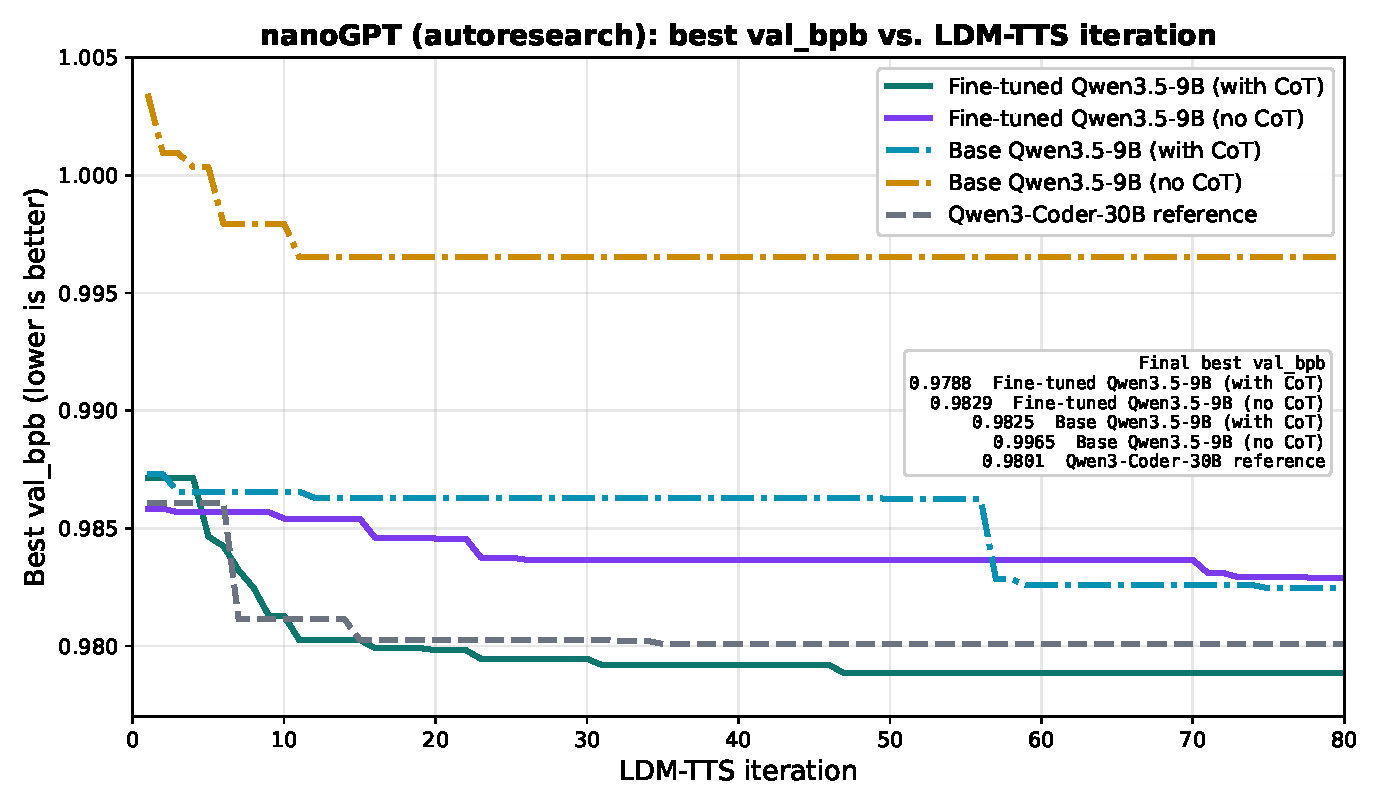
\includegraphics[width=0.92\linewidth]{figure/nanogpt_finetune_cot.pdf}
\caption{\textbf{Reasoning-augmentation ablation on \texttt{autoresearch}.} Best validation bits-per-byte
(lower is better) versus LDM-TTS iteration inside the identical acquisition-guided loop. Discovery fine-tuning
plus reasoning (teal) reaches the lowest \texttt{val\_bpb} and stays below the Qwen3-Coder-30B reference; the
reasoning channel helps both the fine-tuned and base models, and the base model without reasoning stalls early.
Curves are held at their last value once converged.}
\label{fig:nanogpt-finetune-cot}
\end{figure}

\begin{table}[t]
\centering
\small
\begin{tabular}{@{}llccc@{}}
\toprule
\textbf{Weights} & \textbf{Reasoning} & \textbf{\texttt{autoresearch}} & \textbf{Antibody} & \textbf{Small-molecule} \\
 &  & \textbf{val\_bpb $\downarrow$} & \textbf{$-E_{\mathrm{bind}}$ $\uparrow$} & \textbf{Hypervolume $\uparrow$} \\
\midrule
Base Qwen3.5-9B      & off & $0.9965$ & $102.6$ & $16.49$ \\
Base Qwen3.5-9B      & on  & $0.9825$ & $104.4$ & --- \\
Fine-tuned (LDM-SFT) & off & $0.9829$ & $105.1$ & $22.28$ \\
\textbf{Fine-tuned (LDM-SFT)} & \textbf{on} & $\mathbf{0.9788}$ & $\mathbf{105.5}$ & $\mathbf{26.66}$ \\
\midrule
\multicolumn{2}{@{}l}{Qwen3-Coder-30B reference (full schema)} & $0.9801$ & --- & --- \\
\bottomrule
\end{tabular}
\vspace{0.4em}
\caption{\textbf{Cross-domain $2\times2$ reasoning-augmentation ablation.} Base vs.\ discovery-fine-tuned
weights crossed with inference-time reasoning on/off, each evaluated inside the identical acquisition-guided LDM
loop. Metrics: best validation bits-per-byte (lower is better) for \texttt{autoresearch}; KRAS G12D Pareto
hypervolume (higher is better) for small-molecule; and mean negative Absolut binding energy over five antigens
(higher is better) for antibody CDRH3. Across all three domains the reasoning-enabled fine-tuned model attains
the best score, and on \texttt{autoresearch} it further surpasses the larger Qwen3-Coder-30B reference.}
\label{tab:finetune-cot-ablation}
\end{table}

\begin{figure}[t]
\centering
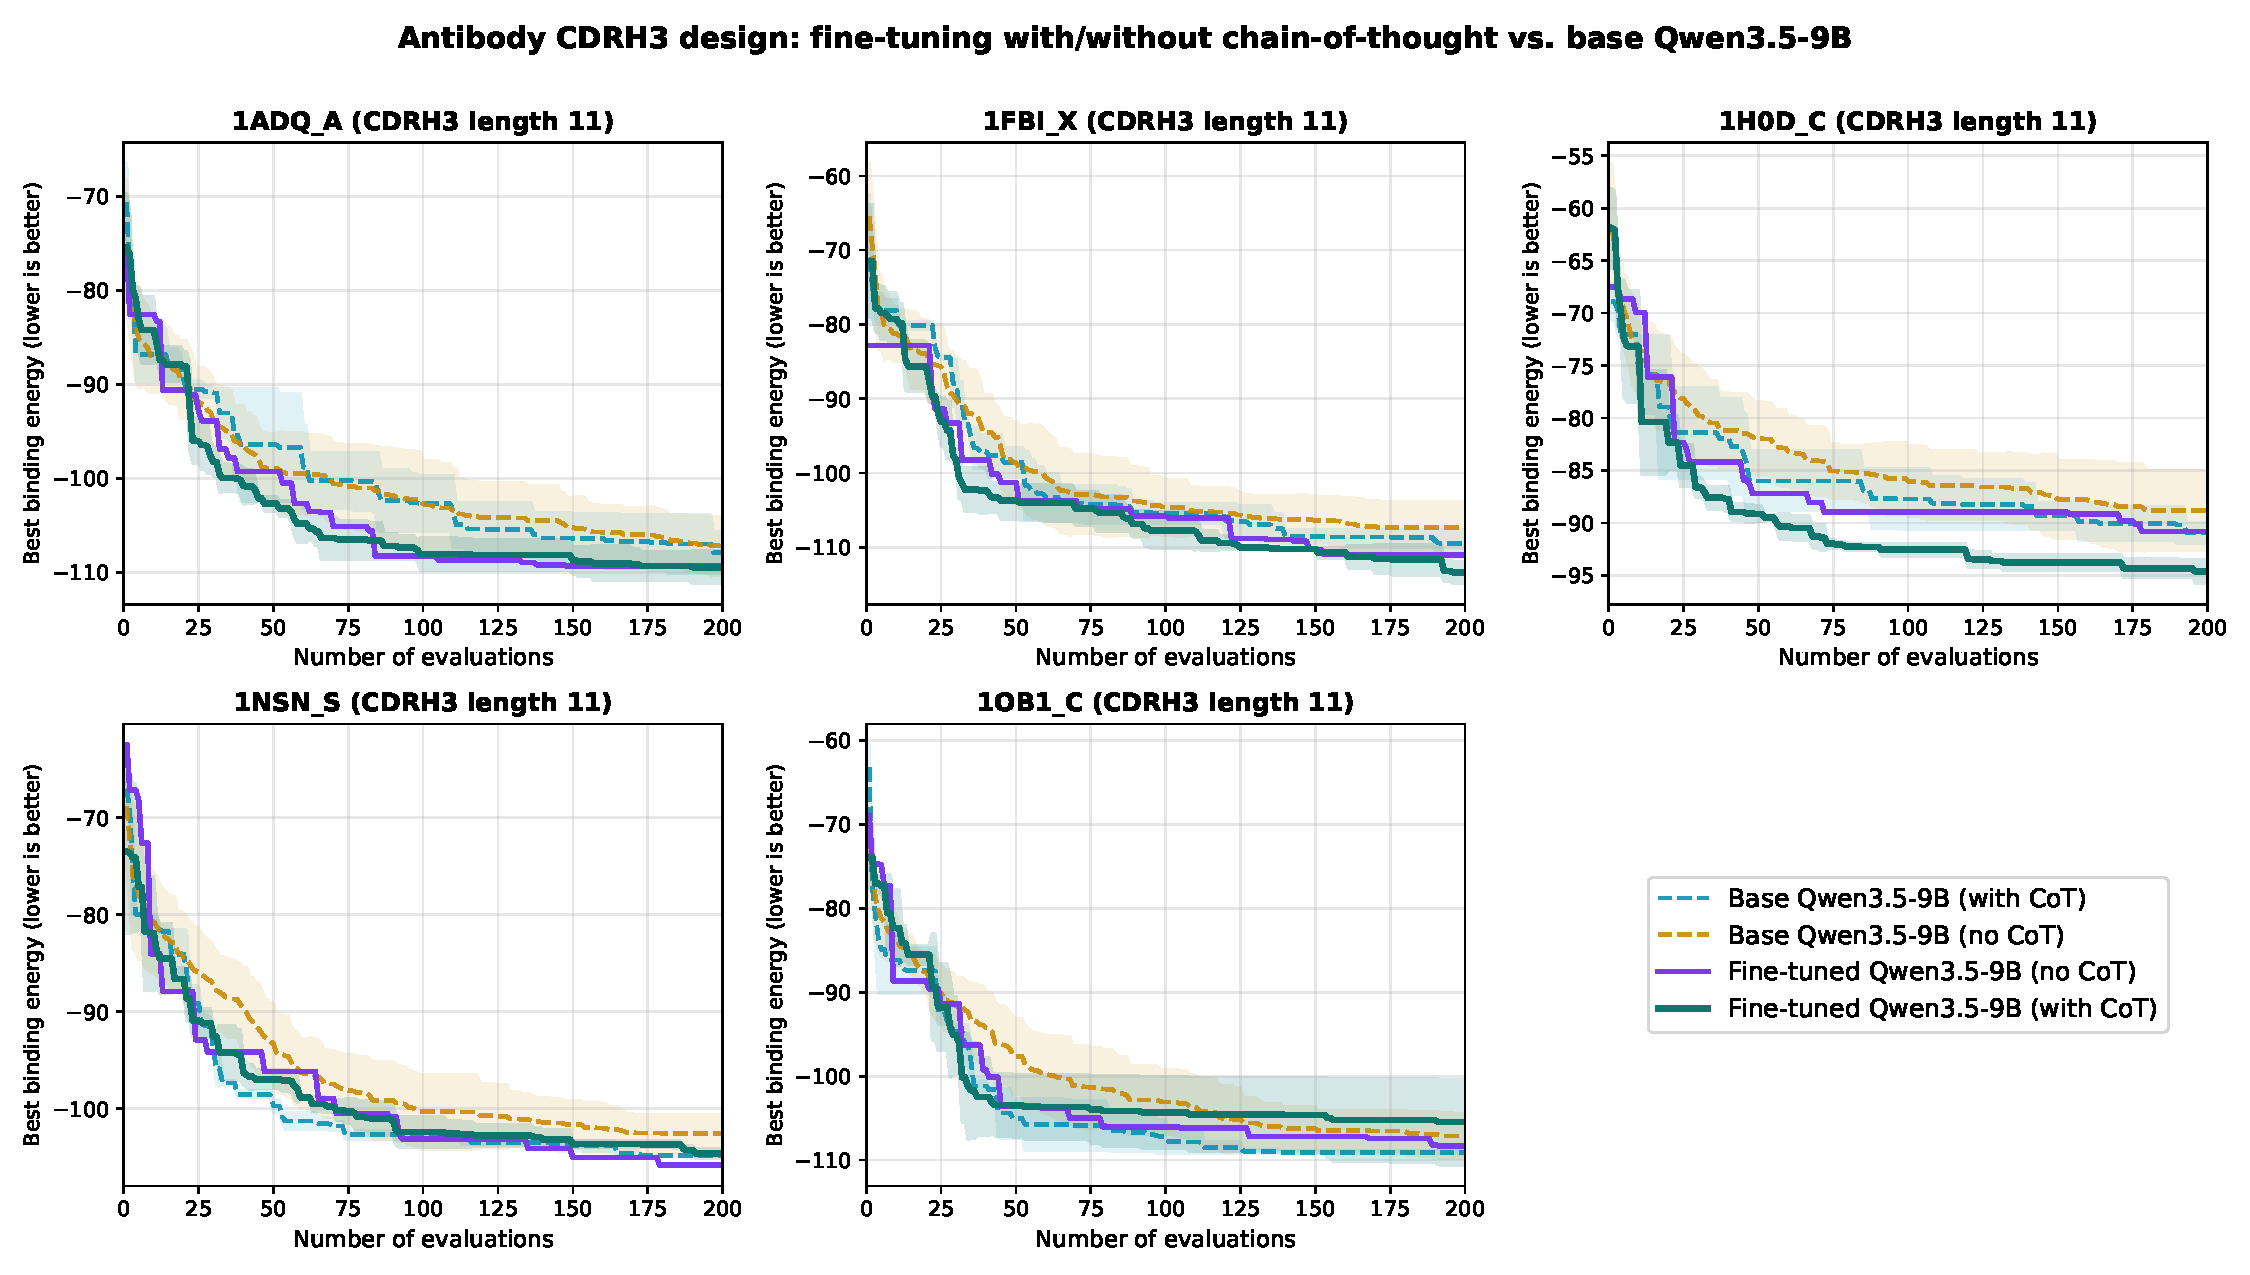
\includegraphics[width=0.95\linewidth]{figure/protein_finetune_cot.pdf}
\caption{\textbf{Antibody CDRH3 design.} Best Absolut binding energy (lower is better) versus number of
evaluations inside the identical acquisition-guided loop (EI acquisition, parallel budget $600$), for five
antigens. Both discovery-fine-tuned variants---with chain-of-thought (teal) and without (purple)---are compared
against base Qwen3.5-9B with and without chain-of-thought (dashed); shaded bands denote mean$\pm$std across
available seeds. Fine-tuning improves over the base model across the antigens, and the reasoning-augmented
fine-tuned model reaches the lowest binding energy on average, attaining the best mean $-E_{\mathrm{bind}}$ of all
four configurations (Table~\ref{tab:finetune-cot-ablation}).}
\label{fig:protein-finetune-cot}
\end{figure}


